\documentclass[../main.tex]{subfiles}

\begin{document}
\onehalfspacing

%UNA MUUUUY HUMILDE INTRODUCCIÓN

%\section{Motivación}

La comunicación es un fenómeno complejo. Esta nace de la necesidad del ser humano por el intercambio efectivo de ideas. Con el avance de la tecnología, se ha ido reduciendo el costo de la mensajería de un contacto lejano, mejorando la calidad de transmisión del mensaje y reduciendo el tiempo de respuesta entre el comunicante emisor y el comunicante receptor [\cite{alhadlaq2016technology}] . Las \textit{redes de medios sociales} (\RMS) son el resultado más reciente de comunicación en medios no tangibles. Sin embargo, el interés político actual de las mismas puede manipular el fin de la comunicación hacia una beneficencia meramente privada o hacia un mérito no loable [\cite{Chen2021}]. Hoy en día, las \RMS han modificado a la sociedad: Ejemplo de ello, el portal LinkedIn ha mostrado una nueva forma de generar y crear líderes para el avance de los negocios\footnote{Osman, M. (2021, July 20). \textit{Mind-Blowing LinkedIn Statistics and Facts (2022)}. Extraído el 10 de enero de 2022 de Kinsta. Sitio web  https://kinsta.com/blog/linkedin-statistics/}. De la misma manera, la sociedad ha podido modificar leyes internas de las \RMS: Twitter notifica a sus usuarios sobre las medidas y restricciones realizadas a través de su blog de su compañía\footnote{\href{https://blog.twitter.com/en\_us/topics/company.html}{Blog oficial de Twitter.} }. 

 %

%MENCIONAR LAS NECESIDADES DE ABARCAR ESTE PROBLEMA (LO ECONOMICO, POLITICO (REDES DE POLITICA) Y SOCIAL. ASÍ COMO UNA NECESIDAD DE MARKETING PARA VENDER UN PRODUCTO A MENOR COSTO.
% AQUI SE PUEDE PONER PORQUE LAS ECUACIONES DIFERENCIAS NO SIRVEN (Y PONER LA CITA AL OTRO CAP[ITULO PARA MAYOR EXPLICACIÓN]


%RELACIONARLO CON EL ENFOQUE DEL PROYECTO. 
% BREVE RESUMEN DE DETALLES, EXPLICAR LA BASE Y EL OBJETIVO. 


\begin{figure}[h!]
    \centering
    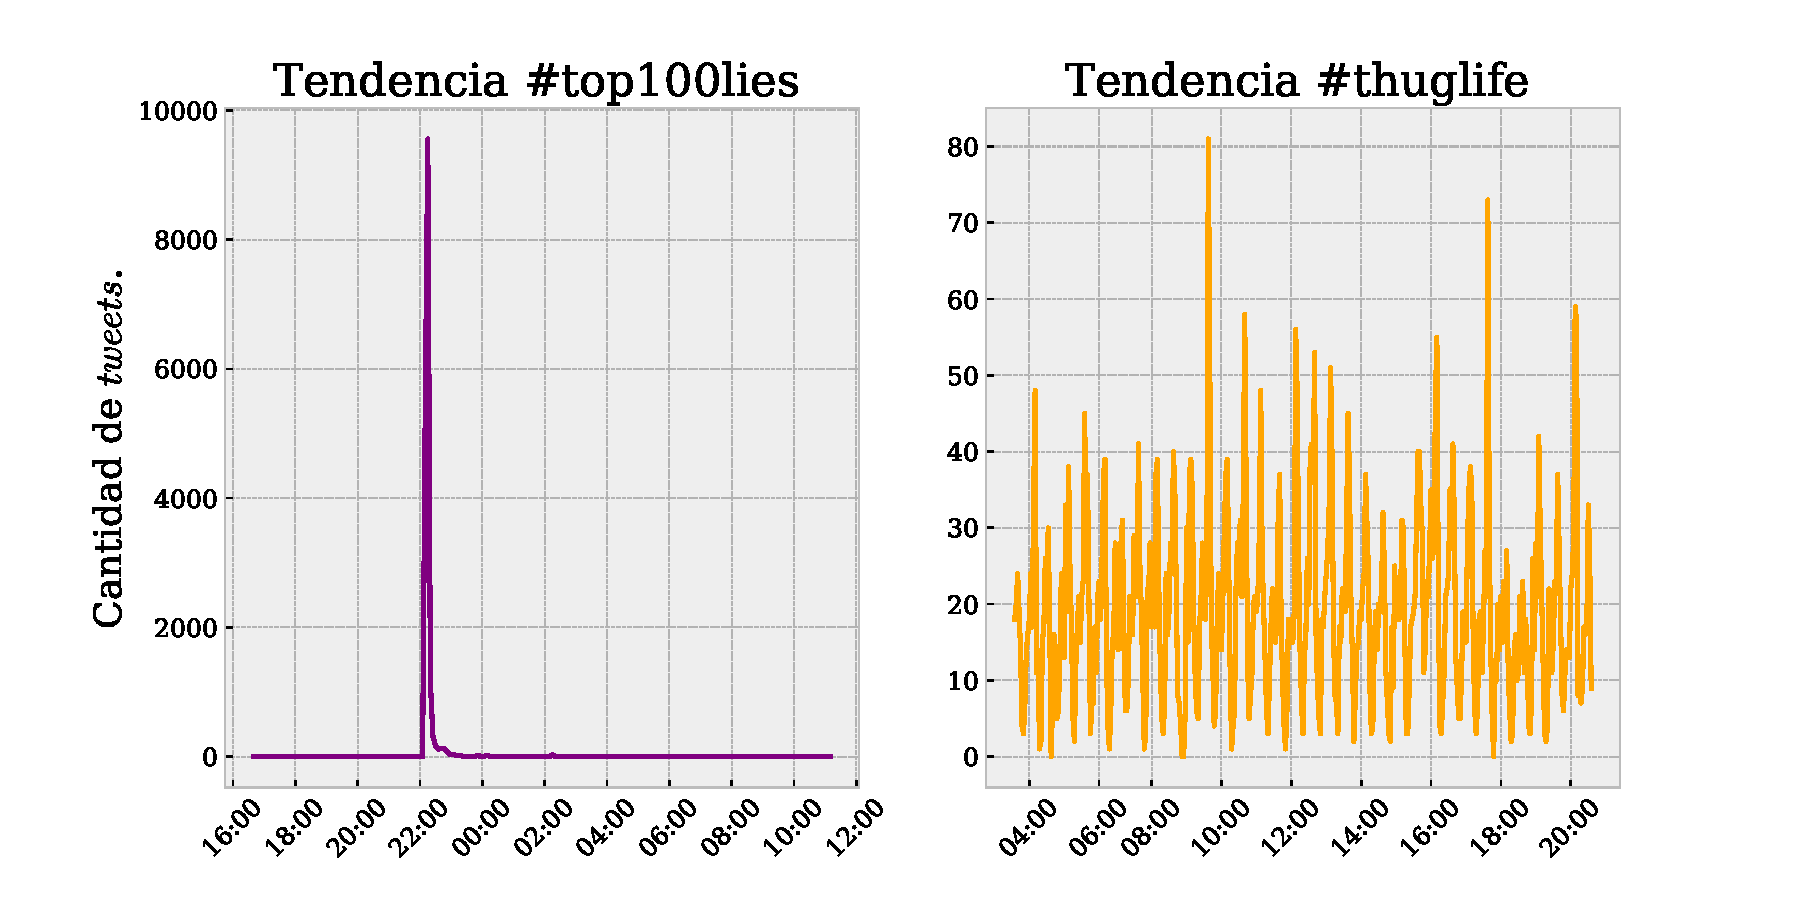
\includegraphics[scale = 0.55]{images/introduction_timeserie.pdf}
    \caption{Series de tiempo de dos tendencias a través del tiempo. En el eje de las ordenadas, se contabiliza la cantidad de interacciones que ocurrieron en el periodo de tiempo marcado por el eje de abscisas. La imagen del lado izquierdo es de comportamiento explosivo debido a la alta interacción en un periodo de tiempo muy corto, mientras que la imagen del lado derecho no lo es debido a su parcial y constante interacción a través del tiempo. Fuente: Elaboración propia.}
    \label{fig:introducction_timeserie_example}
\end{figure}


%El comportamiento mostrado en las \RMS no debe distar de la interacción entre personas.
El ser humano, por su propia naturaleza, toma sus decisiones de forma interna donde lista cada una de sus actividades por orden de prioridad. Esto último, siendo consecuencia de un intento eficiente de asignación de recursos [\cite{Barabsi2005}]. Por lo tanto, no es algo inesperado encontrar diversos patrones y eventos con comportamientos similares a la naturaleza de la comunicación humana. Uno de estos es aquel donde entre periodos largos de tiempo sin interacción, existe un pequeño lapso de tiempo con una alta cantidad de interacciones. A este tipo particular de comportamiento se denomina \textit{comportamiento explosivo} [\cite{oka2014fluctuation}]. Un ejemplo de ello lo podemos ver en la Figura \ref{fig:introducction_timeserie_example}, donde la imagen de lado izquierdo muestra una alta interacción en un lapso inferior a una hora.

Una modelación sencilla de este fenómeno puede verse al considerar dos estados por cada individuo del sistema: Activo e inactivo. Para ello, la población puede fluctuar en una única dirección, es decir, pasar del estado inactivo al activo. Un simple sistema de ecuaciones diferenciales lineales como el siguiente puede representar el fenómeno:

\begin{align*}
    \Dot{x} &= -\alpha xy ,\\
    \Dot{y} &= \alpha xy ,\\
\end{align*}
donde $x$ puede representar nuestra población activa,  $y$ la población no activa y $\alpha$ una tasa de cambio de un estado a otro. La interacción entre las poblaciones está dada por el producto de $x$ con $y$. El significado del producto implica una interacción homogénea entre los individuos y es constante durante el tiempo de análisis. Esta interacción, si bien es simplista en su interpretación, se vuelve imprecisa para detallar interacciones con comportamientos explícitos entre los individuos del sistema. Como consecuencia de esta modelación, se restringe el estudio de la dinámica del sistema considerando el posible impacto de la interacción social de los mismos usuarios. 

Por lo que, el \textbf{objetivo principal} es: Caracterizar el comportamiento explosivo utilizando únicamente la topología del sistema. Para alcanzar el objetivo, se seguirá una metodología basada en redes complejas y analizando una base de tendencias de Twitter que reflejan el comportamiento explosivo. Parte de la bibliografía actual, dedicada a este particular problema, se enfoca en la dinámica de propagación de tipo cascada siguiendo una cadena de interacciones (véase la sección de antecedentes para un mayor detalle). 

% Con base en lo anterior, la siguiente investigación se centrará en esta particular cuestión: ¿Es posible caracterizar este comportamiento explosivo usando únicamente la topología del sistema? Se resolverá esta cuestión 

% siguiendo una metodología basada en redes complejas y analizando una base de tendencias de Twitter que reflejan este comportamiento. Parte de la bibliografía actual dedicada a este particular problema, se enfoca en la dinámica de propagación de tipo cascada siguiendo una cadena de interacciones (véase la sección de antecedentes para un mayor detalle). 

Si bien tenemos que la bibliografía muestra que existe un interés para pronosticar cuando una tendencia pueda exhibir un comportamiento explosivo [\cite{Mathioudakis2010, Keeling2005}], no se  enfocan en la interacción y organización de los usuarios partícipes. Un interés principal en esta problemática parte desde el interés social [\cite{Barabsi2005}], hasta el económico y el político [\cite{Chen2021}].

Este trabajo está organizado como sigue: 

Capítulo 1. Antecedentes. En este capítulo se mostrará un breve panorama de las investigaciones previas en torno al comportamiento explosivo en la dinámica de poblaciones. 

Capítulo 2. Marco teórico.  Se mostrarán los fundamentos teóricos utilizados en este trabajo. Se comienza con teoría de redes y termina con una síntesis de la entropía de Shannon. 

Capítulo 3. Metodología. Se mostrará el procedimiento de la generación de  las redes usadas en el trabajo. Asimismo, se presentan los supuestos principales que llevaron a esta modelación.

Capítulo 4. Análisis y resultados. En este capítulo, se explican los resultados de cada uno de los modelos de redes presentados en el capítulo de metodología.






%%%TODO : Especificar el objetivo
%%%TODO : En el último párrafo explicar como está organizada esta tesis





\end{document}



% EXTRA PART TO ADD IN ANTECEDENTES 

La comprensión de la difusión de un ente, tangible o intangible, en un sistema es un problema de índole complejo: en particular, aquellos dominados por la dinámica de la interacción de humanos [\cite{Miritello2013}]. Los sistemas dinámicos no lineales son pioneros en esta problemática abarcando sus soluciones en función del espacio fase generado al modificar cada uno de los coeficientes del sistema [\cite{Dimitrova2000 }]. Este paradigma introduce un índice del tiempo que muestra la relación explícita de los estados en cada estado del tiempo. Sin embargo, cuenta con la sutil problemática en desvanecer la estructura topológica de la interacción de los individuos del sistema al considerar todas las relaciones iguales entre la población [\cite{Keeling2005}]. En esencia, son modelos interesados en la razón de cambio entre los estados que la interacción en sí. 

Dado que estas ecuaciones abstraen la relación de intercambio de individuos en los estados de interés, se puede extrapolar dicha moción para el caso de intercambio de ideas y opiniones [\cite{Dimitrova2000 }]. Entre estos sistemas, las \RMS social son un buen medio para analizar la dinámica entre comunicantes debido a la sencillez de conectividad y reacción inmediata ante sucesos espontáneos, además de la amplia y basta cantidad de información. 

Ejemplo de estas, quizá las más llamativa y conocida, es la plataforma \textit{Twitter}. Dicha plataforma cuenta con 192 millones de usuarios activos diariamente\footnote{Ying Lin. (2021). \textit{10 Twitter statistics every marketer should know in 2021}. 1 de noviembre de 2021, de Oberlo Sitio web: https://www.oberlo.com/blog/twitter-statistics}. En esta \RMS, podemos encontrar cuatro sencillas acciones entre usuarios:

\begin{itemize}
    \item \textit{Tweet}. 
    
    Es la acción de un usuario por publicar una idea u opinión. Se puede presentar como un texto plano o con añadidos como \textit{emojis}, \textit{emoticons} o archivos audiovisuales. 
    
    \item \textit{Follow}. 
    
    Es la acción de un usuario $A$ para seguir a un usuario $B$. Esta es la primera relación entre los usuarios. Esta acción permite al usuario $A$ recibir notificaciones de la actividad del usuario $A$.
    % \textit{A priori}, es una manera sencilla de representar gustos afines entre los usuarios. Claramente, cuando hay seguimiento mutuo (siguiendo de nuestro ejemplo, cuando $B$ sigue a $A$ también), entonces esta relación se vuelve más fuerte.  
    
    \item \textit{Retweet}. 
    
    Es la acción de un usuario $A$ por publicar un \textit{tweet} existente de algún usuario $B$ y  publicarlo en el perfil de $A$ con el nombre de $B$.
    Es, en términos sencillos, citar la idea u opinión de un usuario para apoyarla. 
    
    \item \textit{Mention}. 
    
    Es la acción de un usuario $A$ por \textit{tweetar} algún contenido etiquetando o mencionando a otro usuario $B$. Es una comunicación directa de $A$ a $B$.
    
\end{itemize}


Por su propia dinámica, se ha hecho de un espacio común de choque político, social y cultural. En consecuencia, esta comunicación no visible ha generado desde  eventos no deseables\footnote{Hudson, John. \textit{The Most Infamous Terrorists on Twitter.}”, The Atlantic, 1 de noviembre de 2021, de The Atlantic. Sitio web: \href{https://www.theatlantic.com/international/archive/2012/01/most-infamous-terrorists-twitter/333662/}{Link}.} hasta  sucesos beneficiosos para la comunidad\footnote{Santolini, Marc. \textit{Covid-19: The Rise of a Global Collective Intelligence?}, 17 de enero de 2021, de The Conversation. Sitio web: \href{http://theconversation.com/covid-19-the-rise-of-a-global-collective-intelligence-135738}{Link}. }. Esto llevó al análisis de \textbf{tendencias} (\textit{trends}). En específico, una tendencia es un tema, idea o suceso que se es muy discutido entre los usuarios. Puede estar presente de diversas formas como \textit{memes}, videos o texto. 
Bajo este nulo conocimiento sobre el comportamiento y consecuencias de alguna tendencia, Twitter notifica a sus usuarios sobre las medidas y restricciones realizadas a través de su blog de compañía \footnote{\href{https://blog.twitter.com/en\_us/topics/company.html}{Blog oficial de \textit{Twitter}.}}.

%Definir con ejemplos lo que es el comportamiento explosivo. 

%TODO : COLOCAR CITAS DE EJEMPLOS 
Si bien se han reportado diversos fenómenos con el mismo tipo de comportamiento desde enfoques sociales [citas sociales] y médicos [colorcar citras de ejemplos] , en todas estas escala ocurre que 

% \begin{figure}
%     \centering
%     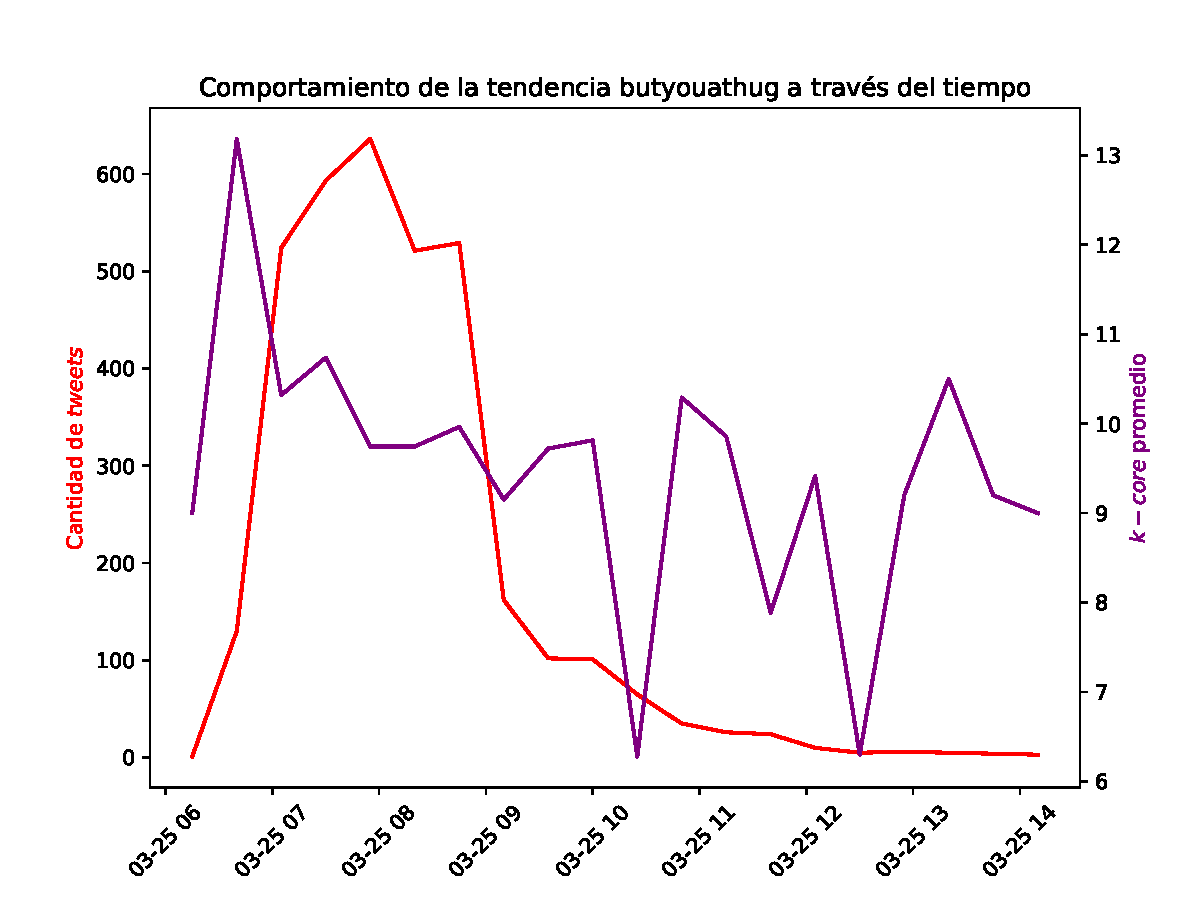
\includegraphics[scale = 0.7]{images/ejemplodecomportamientocore.pdf}
%     \caption{Visualización de una tendencia con comportamiento explosivo. Notemos como el intervalo de interacción máxima ($t^{*}$) es entre las 7 y 8 horas del día 25 de marzo. Sin embargo, el $k-core$ promedio de los usuarios que inician la comunicación antes de ese periodo de tiempo tiene un crecimiento en su $k-core$ bastante significativo (ver marco teórico).}
%     \label{fig:introduccion_comportamientprevio}
% \end{figure}

En el presente trabajo, se aborda un análisis de la dinámica de difusión de información, como un símil a la propagación de una enfermedad, en función de la topología de las relaciones entre los comunicantes. Como estudio objetivo, se enfoca en aquellas tendencias cuyo comportamiento es de caracter explosivo. 

% entre los comunicantes ocurre de manera masiva en un lapso de tiempo muy corto.  

Los modelos presentes en el escrito se basan en diversos artículos que abarcan este problema en diversas escalas. Por un lado, tenemos una escala local donde se énfasis en la vecindad de los comunicantes activos [\cite{Model_Pramanik2017,Model_Fabrega_regresion,D_weng2014predicting,Model_retweets_inproceedings}]; Por otro lado, donde el modelo anterior se escala a comunidades viendo la interacción de los verdaderos comunicantes en ellas [\cite{Dong2017,Chng2015_bottom-up}]. De ambos modelos, se les aplicaran métricas de centralidad y métricas globales para encontrar una diferencia entre las tendencias de comportamiento explosivo. Finalmente, se presentará un árbol de clasificación binaria del comportamiento entre 25 y 50 minutos antes del comportamiento explosivo. Dicho algoritmo tiene una calificación F1  (\textit{F1-score}) del 0.80.

Dichos análisis serán realizados con una base de datos recabada del portal \textit{Twitter} con una fecha de extracción del 24 de marzo de 2012 hasta el 26 de abril de 2012. Dicha base cuenta con varios \textit{tweets} agrupados por su tendencia. 
Esta base de datos se puede encontrar en el portal oficial del Centro de Investigación de Redes y Sistemas Complejos (\href{https://cnets.indiana.edu/about/}{CNetS}). 


\begin{figure}[h!]
    \centering
    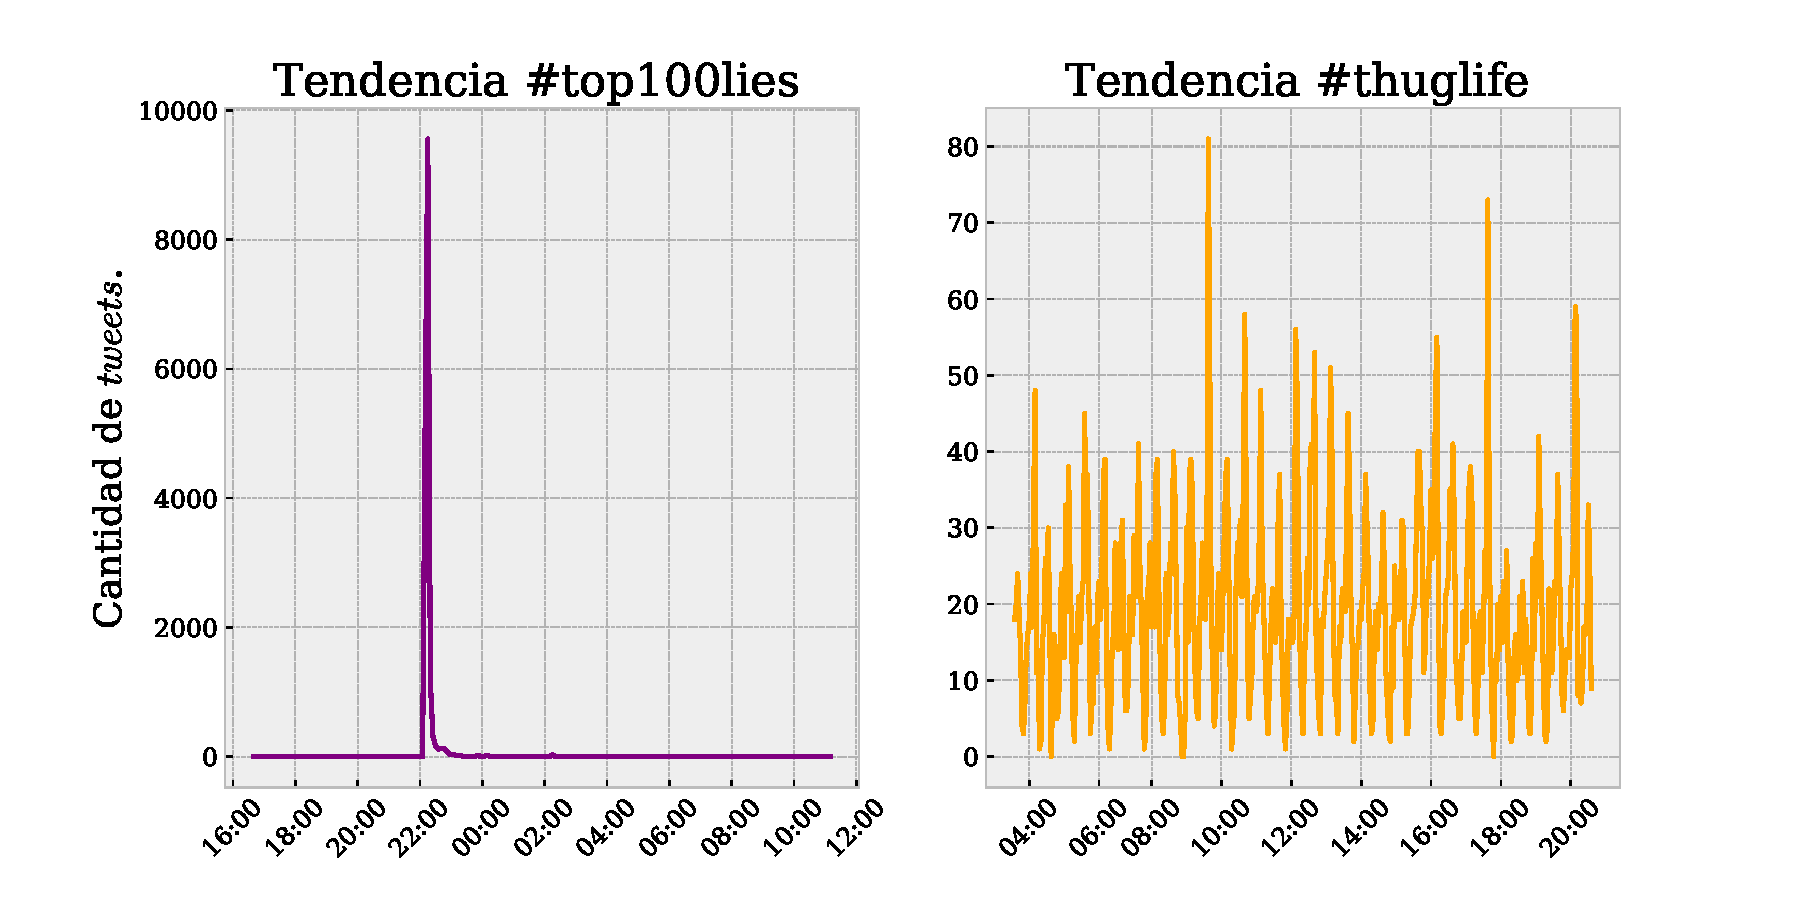
\includegraphics[scale = 0.55]{images/introduction_timeserie.pdf}
    \caption{Serie de tiempo de dos tendencias a través del tiempo. La imagen lado izquierdo es de comportamiento explosivo. Nótese el inesperado cambio de la actividad }
    \label{fig:introducction_timeserie_example}
\end{figure}

\addcontentsline{toc}{section}{Objetivo}  
\section*{Objetivo}

% Obtener un patrón de los comunicantes  generado por los usuarios partícipes de tendencias con comportamiento explosivo. 
Identificar tendencias con comportamiento explosivo en función de la red social de los usuarios partícipes.